%%%%%%%%%%%%%%%%%%%%%%%%%%%%%%%%

\documentclass[11pt,a4paper]{article}
\usepackage{times}
\usepackage[utf8]{inputenc}
\usepackage[croatian]{babel}
\usepackage[T1]{fontenc} % Latin Modern

%%%%%%%%%%%%%%%%%%%%%%%%%%%%%%%%


%%%%%%%%%%%%%%%%%%%%%%%%%%%%%%%%
%%%%%%%%  MATEMATICKI PAKETI %%%%%%%%%%%
%%%%%%%%%%%%%%%%%%%%%%%%%%%%%%%%

\usepackage{amsmath}
\usepackage{amsfonts}
\usepackage{amssymb}
\usepackage{esvect}

%%%%%%%%%%%%%%%%%%%%%%%%%%%%%%%%

%%%%%%%%%%%%%%%%%%%%%%%%%%%%%%%%
%%%%%%%%%% PAKETI ZA SLIKE  %%%%%%%%%%%%
%%%%%%%%%%%%%%%%%%%%%%%%%%%%%%%%

\usepackage{graphicx}
\usepackage{float}
\usepackage[hidelinks]{hyperref}
\usepackage{caption}
\usepackage{subcaption}
\usepackage{booktabs}


%%%%%%%%%%%%%%%%%%%%%%%%%%%%%%%%

%%%%%%%%%%%%%%%%%%%%%%%%%%%%%%%%
%%%%%%%%%    PRORED 1.5   %%%%%%%%%%%%%%
%%%%%%%%%%%%%%%%%%%%%%%%%%%%%%%%

\renewcommand{\baselinestretch}{1.5}

%%%%%%%%%%%%%%%%%%%%%%%%%%%%%%%%


%%%%%%%%%%%%%%%%%%%%%%%%%%%%%%%%
%%%%%%%%%% TABLICA - ANTUN %%%%%%%%%%%%
%%%%%%%%%%%%%%%%%%%%%%%%%%%%%%%%

\usepackage{array}
\usepackage{multirow}
\newcolumntype{C}[1]{>{\centering\let\newline\\\arraybackslash\hspace{0pt}}m{#1}}
\newcolumntype{L}[1]{>{\raggedright\let\newline\\\arraybackslash\hspace{0pt}}m{#1}}
\newcolumntype{R}[1]{>{\raggedleft\let\newline\\\arraybackslash\hspace{0pt}}m{#1}}
\usepackage{ctable}

%%%%%%%%%%%%%%%%%%%%%%%%%%%%%%%%

%%%%%%%%%%%%%%%%%%%%%%%%%%%%%%%%
%%%%%%%%%% TABLICA - MARTINA %%%%%%%%%%%
%%%%%%%%%%%%%%%%%%%%%%%%%%%%%%%%

\makeatletter
\renewcommand*\env@matrix[1][\arraystretch]{%
  \edef\arraystretch{#1}%
  \hskip -\arraycolsep
  \let\@ifnextchar\new@ifnextchar
  \array{*\c@MaxMatrixCols c}}
\makeatother



%%%% LATEX KOD ZA KORISTENJE TABLICE %%%%
%%% PRIMJER %%%

%\setlength\extrarowheight{1pt}
%\begin{table}[h]
%\centering
%\caption{Tablica s prikazom }
%\label{prva}
%\begin{tabular}{|l|c|}
%\hline
%\textbf{txt} &  \\ \hline 
%txt & txt    \\ 
%txt & txt   \\ \hline
%txt & txt    \\ \hline
%\end{tabular}
%\end{table}

%%%%%%%%%%%%%%%%%%%%%%%%%%%%%%%%


%%%%%%%%%%%%%%%%%%%%%%%%%%%%%%%%
%%%%%%% DIO ZA UNOS ISJECAKA KODA %%%%%%%%
%%%%%%%%%%%%%%%%%%%%%%%%%%%%%%%%

\usepackage{listings}
\usepackage{color}
 
\definecolor{codegreen}{rgb}{0,0.6,0}
\definecolor{codegray}{rgb}{0.5,0.5,0.5}
\definecolor{codepurple}{rgb}{0.58,0,0.82}
 
\lstdefinestyle{mystyle}{   
    commentstyle=\color{codegreen},
    keywordstyle=\color{blue},
    numberstyle=\tiny\color{codegray},
    stringstyle=\color{codepurple},
    basicstyle=\footnotesize,
    breakatwhitespace=false,         
    breaklines=true,                 
    captionpos=b,                    
    keepspaces=true,                 
    numbers=left,                    
    numbersep=5pt,                  
    showspaces=false,                
    showstringspaces=false,
    showtabs=false,                  
    tabsize=1
}
 
\lstset{style=mystyle}

%\lstinputlisting[language=Matlab, firstline=1, lastline=4, numbers=left, frame=single, label={lst:prvi}, caption={Diskretizacija sustava korištenjem Matlaba}, captionpos=b]{peti.m} 

%%%%%%%%%%%%%%%%%%%%%%%%%%%%%%%%


%----------------------------
% za uredjenje stranice
\usepackage[left=2.5cm,right=2.5cm,top=2.5cm,bottom=2.5cm]{geometry}
\usepackage{fancyhdr}
\pagestyle{fancy} 
\lhead{\leftmark}
\rhead{\rightmark}
\usepackage{titlesec} %za točku iza broja sectiona
\titleformat{\section}{\huge\bfseries}{\thetitle.\quad}{0em}{}
\titleformat{\subsection}{\LARGE\bfseries}{\thetitle.\quad}{0em}{}
\titleformat{\subsubsection}{\Large\bfseries}{\thetitle.\quad}{0em}{}
\titleformat{\paragraph}
{\normalfont\large\bfseries}{\thetitle.\quad}{1em}{}
\titlespacing*{\paragraph}
{0pt}{3.25ex plus 1ex minus .2ex}{1.5ex plus .2ex}
\setcounter{secnumdepth}{5}

\usepackage{indentfirst} %uvlacenje prvog paragrafa
% primjer pozivanja sectiona
% \section*{UVOD} \pdfbookmark{UVOD}{section:UVOD}

\usepackage{tocloft}
\usepackage{import}
\usepackage{standalone}
\graphicspath{{Uvod/}, {Ciljevi/}, {Materijal/}, {Rasprava/}, {Rezultati/}} 

\hypersetup{
  colorlinks   = true, %Colours links instead of ugly boxes
  urlcolor     = black, %Colour for external hyperlinks
  linkcolor    = black, %Colour of internal links
  citecolor   = blue %Colour of citations
}

\usepackage{subcaption}
\usepackage{lscape}
\begin{document}


CAD MODEL mehaničke konstrukcije - BRUNO

U ovom poglavlju je opisana mehanička konstrukcija letjelice. Osnova je postojeća laboratorijska letjelica ARDUCOPTER. Letjelica ARDUCOPTER je standarnog dizajna, s četiri pogonska $brushles DC$ motora s pripadnim $ESC$ pogonima. Zbog jednostavnog dizajna, vrlo je jednostavno raditi razne promjene i dodavati razne upravljačke uređaje, senzore i aktuatore. U laboratoriju trenutno postoji nekoliko modela letjelica ovog tipa koje se koriste za većinu eksperimenata. Dizajn i veličina letjelice je prikladna za sve eksperimente koji se provode u laboratoriju, uključujući planiranje i izvođenje trajektorija u prostoru, manipulaciju objekata i drugo. Upravo zato odlučeno je modificirati jednu od postojećih konstrukcija te izraditi platformu za eksperimentalno testiranje novog koncepta upravljanja višerotorskom letjelicom. Glavna modifikacija se odnosi na dizajniranje i izradu mehanizma kojim će se omogućiti pomak mase na kraku. Također, potrebno je smjestiti sve ostale komponente nužne za upravljanje letjelicom, poput kontrolera leta i upravljačkog sklopovlja pomičnih masa.

\begin{figure}[h!]
	\centering
	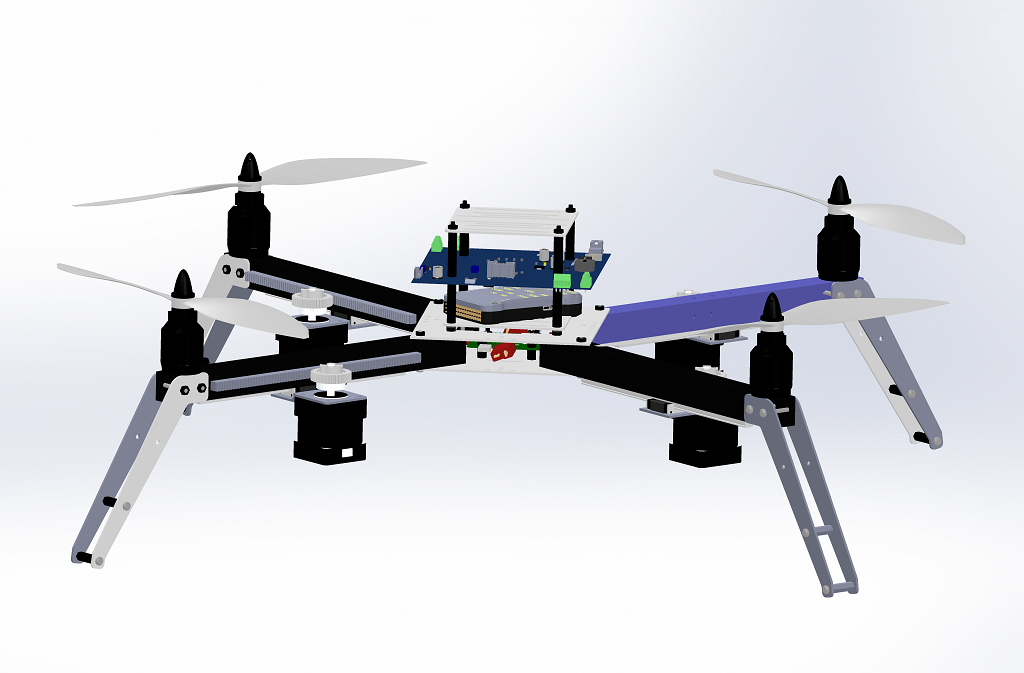
\includegraphics[width=0.9\textwidth]{figures/arducopter_with_PCB.png}
	\caption{3D model modificirane letjelice ARDUCOPTER}
	\label{Slika:3D_drone_final}
\end{figure}

\subsection{Letjelica ARDUCOPTER}

Osnova konstrukcije letjelice s pomičnim masama je višerotorska letjelica ARDUCOPTER, prikazano slikom \ref{Slika:3D_drone_original}. ARDUCOPTER je laboratorijska letjelica pogonjena s 4 $brushless DC$ motora. Koncept upravljanja je klasični, brzom promjenom brzina vrnje motora, ostvaruju se zadani kutevi i kutne brzine letjelice. Letjelica ima jednostavan dizajn, što omogućava jednostavne nadogradnje, poput različitih upravljačkih uređaja, senzora i aktuatora. Sva proširenja letjelice se jednostavno dodaju jedno iznad drugog na već predviđene položaje iznad razine krakova u centru letjelice. Zbog svega navedenog, ARDUCOPTER je odabran osnovna platforma za izradu višerotorske letjelice s pomičnim masama.


Postojeća mehanička konstrukcija letjelice ARDUCOPTER se u potpunosti koristi, a obuhvaća: 
\begin{center}
	\begin{itemize}
		\item Tijelo letjelice uključujući razvodnu ploču za napajanje iz baterije i prihvat slojeva za proširenje
		\item 4 aluminijska kraka
		\item 4 plastična zaustavna kraka
		\item 4 $brushless DC$ motora s pripadnim $ESC$ pogonima
		\item 4 plastična propelera
	\end{itemize}
\end{center}

\subsubsection*{Modifikacija postojeće letjelice}
Predstavljenu postojeću letjelicu ARDUCOPTER potrebno je modificirati na sljedeći način:
\begin{center}
	\begin{itemize}
		\item Dodati 4 pokretne mase, odabrati aktuatore, konstruirati i izraditi mehanizam kretanja mase po kraku letjelice.
		\item Dodati kontroler leta PIXHAWK PX4, za kompletno upravljanje letjelicom s pokretnim masama
		\item Izraditi elektroničko slopovlje potrebno za pogon masa, realizirati komunikaciju s kontrolerom leta te dodati mogućnosti za daljnja funkcionalna proširenja letjelice.
	\end{itemize}
\end{center}


\begin{figure}[h]
	\centering
	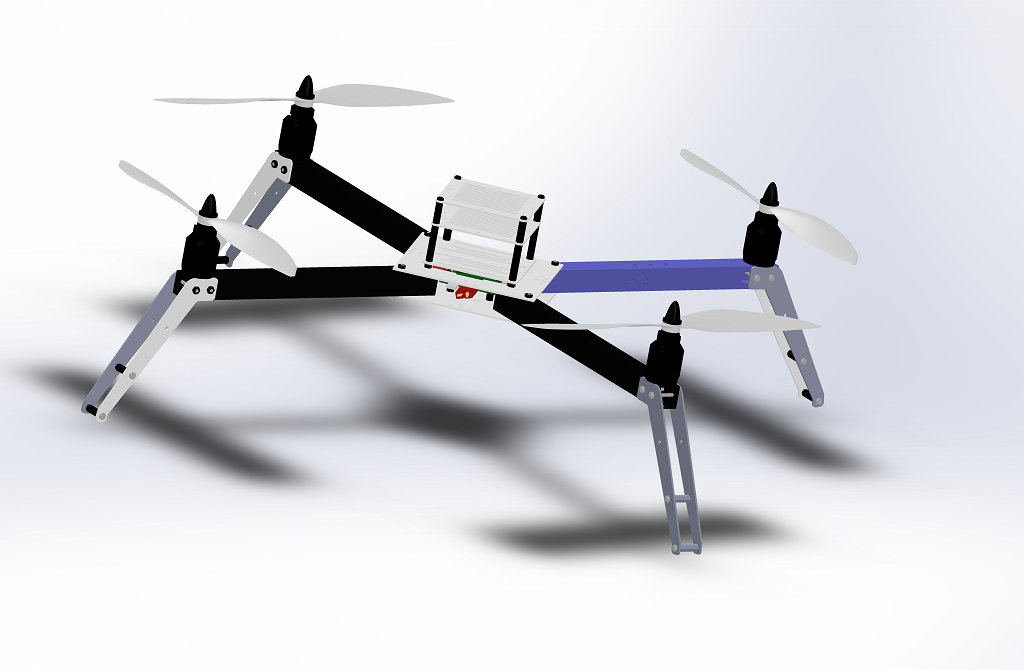
\includegraphics[width=0.9\textwidth]{figures/arducopter_original.png}
	\caption{3D model postojeće letjelice ARDUCOPTER}
	\label{Slika:3D_drone_original}
\end{figure}

\subsection{Klizni mehanizam pokretne mase}

Budući da se novi koncept upravljanja letjelice zasniva na promjeni centra mase, koje je realizirano pomičnim masama na krakovima, potrebno je izraditi mehanizam kretanja pokretne mase po kraku letjelice. Kretanje pomične mase je linijsko, a mehanizam kretanja mora biti realiziran s minimalnim trenjem. Kretanje pokretne mase je ostvareno električnim aktuatorom.

\subsubsection{Aktuator}
Zadaća aktuatora za pokretnu masu je gibanje mase po kraku letjelice, čime se ostvaruje promjena centra mase letjelice. Kako bi ukupna masa letjelice bila manja, fizička masa aktuatora na svakom kraku se koristi kao pokretna masa. Za aktuator je odabran koračni motor POL, prikazan slikom \ref{Slika:stepper_motor}.

\begin{figure}[h!]
	\centering
	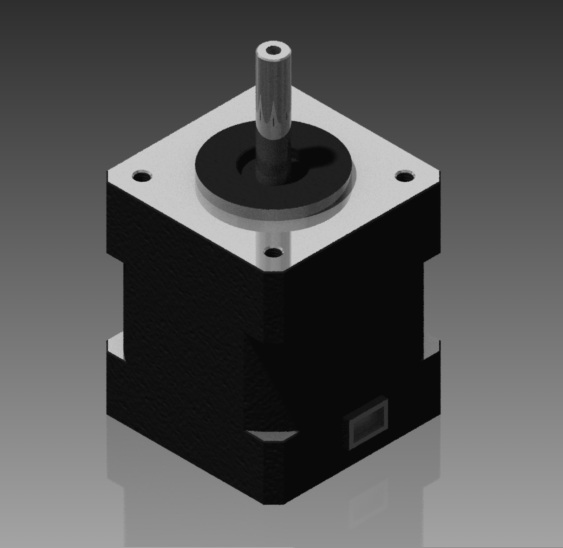
\includegraphics[width=0.3\textwidth]{figures/StepperMotor.jpg}
	\caption{Koračni motor}
	\label{Slika:stepper_motor}
\end{figure}


\begin{table}[h]
	\centering
	\caption{Specifikacije koračnog motora }
	\label{prva}
	\begin{tabular}{|l|c|}
		\hline
		\textbf{Veličina} & 35mm x 35mm x 36mm, neuključujući osovinu  \\ \hline 
		\textbf{Masa} & 180 g  \\ \hline 
		\textbf{Promjer osovine} & 5 mm \\ \hline 
		\textbf{Broj koraka po okretu} & 200 \\ \hline 
		\textbf{Broj faza} & 2 \\ \hline 
		\textbf{Current rating} & 1A po fazi \\ \hline 
		\textbf{Moment zadržavanja} & 1.4 $kg/cm$ \\ \hline 
		\textbf{Moment inercije rotora} & 14 $g/cm^2$ \\ \hline 
	\end{tabular}
\end{table}


\subsubsection{Klizni mehanizam}

\subsubsection{Zupčasti prijenos}


\subsection{Izrada dijelova}

\subsection{Položaj upravljačkog sklopovlja}


\end{document}